% !TeX encoding = UTF-8
% !TeX spellcheck = it_IT
% !TeX root = main.tex

\section{Descrizione dei tag}

\subsection{Richiesta economica}

\subsection{Persone e ruoli}
Uno dei principali obiettivi del sistema è l'individuazione di persone e dei ruoli che esse svolgono nella procedura fallimentare, ovviamente basandoci su ciò che troviamo all'interno dei moduli di richiesta.

Nei vari modelli di richiesta abbiamo individuato principalmente tre entità da poter ritrovare: \fbox{giudice}, \fbox{soggetto} e \fbox{curatore}.
Il primo è spesso individuato ad inizio documento, nell'intestazione, come destinatario della richiesta.
Il soggetto della richiesta è colui che la produce e la firma, spesso preceduto dalla parola ``sottoscritto'' e dalla sua presenza in calce.

Di seguito lo schema delle dipendenze dei tag per le persone e i loro ruoli.

\begin{figure}[H]
\centering
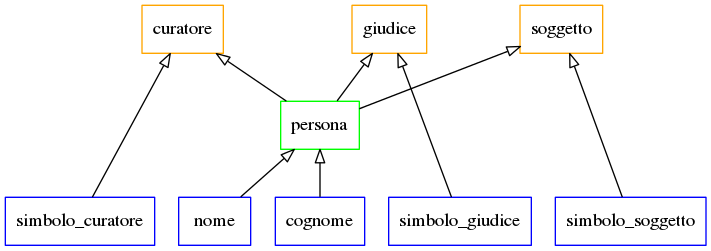
\includegraphics[width=.7\textwidth]{img/persona.png}
\label{fig:persona}
\caption{Schema delle dipendenze dei tag per le persone e i loro ruoli}
\end{figure}

Nell'operazione di tagging vengono ricercati i simboli peculiari delle tre entità, ossia i token che contengono parole chiave da noi precedentemente individuate.
Il tag \verb|parola(giudice)|, ad esempio, introdurrà un \fbox{simbolo\_giudice}. \emph{Sottoscritto} o \emph{sottoscritta}, introdurranno un \fbox{simbolo\_soggetto} mentre \emph{curatore} determinerà un \fbox{simbolo\_curatore}.

Ciascuno di questi tre, associati ad un \verb|tag| \fbox{persona}, costituirà l'entità target che cercavamo in partenza.

Il tag persona merita un discorso a parte.
Il tag \fbox{persona} nasce dalla presenza di \fbox{nome} e \fbox{cognome} in entrambe le permutazioni.
Per questi ultimi 2 tag abbiamo effettuato una ricerca online di diversi database di nomi e cognomi italiani, fondendoli in un file Prolog \verb|persona_kb.pl|, consultato e utilizzato dal modulo \verb|persona|.

Abbiamo previsto la possibilità che ci siano nomi e cognomi composti. La legge italiana stabilisce un limite massimo di 3 nomi e 2 cognomi.
Le regole, di conseguenza, valuteranno come possibili nomi/cognomi sia le singole parole che corrispondono a voci del database, sia a parole concatenate (fino a 3/2), ciascuna delle quali è un possibile nome/cognome.

Ad esempio, prendendo in considerazione delle generalità abbastanza complesse come: ``Simone Addario Chieco'', il sistema ritroverà tanti possibili cognomi:

\begin{prologcode}
cognome('Simone').
cognome('Addario').
cognome('Chieco').
cognome('Simone Addario').
cognome('Addario Chieco').
\end{prologcode}

ma un solo nome

\begin{prologcode}
nome('Simone').
\end{prologcode}

L'unica persona identificata sarà, dunque, l'unica possibile, cioè con nome ``Simone'' e cognome ``Addario Chieco''.

In casi fortemente ambigui, però, come ad esempio ``Cataldo Roberto'' (entrambe le parole possono essere sia nomi o cognomi), il sistema non sarà in grado di disambiguare. Ritroverà la persona Cataldo/Roberto e la persona Roberto/Cataldo. Tuttavia, senza disporre di ulteriore conoscenza sulla persona, questo rimane un compito impossibile anche per l'essere umano.

\subsection{}

\subsection{Mail}
